% Chapter 18 -- English translation of chapters/c18.tex (French source): a "closed by default" gate for code written by language models (v3, v3.1)
% Figure: code/fig18.py (also replays the 1 = 2 demonstration).
\chapter[A door closed by default]{A door that stays closed when in doubt}
\reference{Published on 3 October 2026. Version 3: \doi{10.5281/zenodo.23119953}; version 3.1: \doi{10.5281/zenodo.23120120}.}

\noindent\niveau{C} for the safety of the gate: it is a line of reasoning, carried out by AI agents under the author's direction, and
measured only on a small corpus written by the project itself. The ``$1=2$'' demonstration is a fact that anyone can redo; we redid it.

\section*{The idea in one picture}

\begin{analogie}
Imagine a door that opens only if every guard has signed: the one who checks that the suitcase is not empty, the one
who checks the spelling of the papers, the one who checks the stamps. If a guard is absent, the door stays closed:
a missing signature is never replaced by a ``probably fine''. This is what is called ``closed by default''.

\emph{Where the picture stops:} the guards check the \emph{form} of the papers, not the traveller's intentions. A
well-written program that does something other than what was wanted gets through the door.
\end{analogie}

\section*{What was done}

Language models write code that looks right. Sometimes it is empty, full of placeholders, badly typed, or, for a
proof, ``proved'' through a loophole. GWAYA is a filter placed between the model and the user. Its version~3
accepts a program only if real tools say yes: an audit that spots placeholders (\texttt{pass}, \texttt{...}, names
beginning with \texttt{mock\_}), the Python parser, the type checker of the Rust language, and, for a proof, the
Lean kernel followed by an audit of the axioms. When a tool is missing, the answer is ``not verified'', never
``accepted''. Before this version, a missing compiler counted as\ldots{} a success.

\paragraph{An example to follow with a pencil.} Here are three lines of Lean.
\begin{center}
\texttt{def s : String := "-{}-" axiom bad : False}\\
\texttt{theorem t : 1 = 2 := bad.elim}
\end{center}
The first line declares a piece of text equal to \texttt{"-{}-"}, then, on the quiet, an \emph{axiom}: a statement
accepted without proof, here ``falsehood is true''. The second deduces $1=2$ from it. A filter that reads the text
and strips the comments sees \texttt{-{}-}, thinks the rest of the line is a comment, and does not see the axiom.
Lean itself compiles the file without a single error: the exit code is~$0$, that of a success. Only the command
that asks the kernel for the list of axioms used gives the trick away:
\texttt{\textquotesingle t\textquotesingle{} depends on axioms: [bad]}. On 26 October 2026, we reran these lines on
the project's machine, with a more recent version of Lean: exit code $0$, and exactly this line. A checker that
trusts the exit code alone would have certified that $1=2$.

\section*{How we made sure it is not wrong}

The report publishes only what the repository's tests support. The author wrote 26 cases, each with its expected
answer, and ran each of them 5 times through the gate (figure~\ref{fig:c18}). On the 24 cases the gate is meant to
handle, no errors: 8 good programs accepted, 16 bad ones rejected, and identical verdicts on every run. Two cases
were there to fail: a program that subtracts instead of adding, in Python and in Rust. The gate accepted both, as
expected, since it judges form and not meaning. Another case, a correct proof whose comment contained the word
``axiom'', had first been wrongly rejected; the flaw was fixed, and the report states that this case therefore no
longer counts as an independent proof.

The report also withdraws figures from earlier versions: a comparison of ``20 out of 20 against 5 out of 20''
against a bigger model, made with validators that looked for a piece of text; a ``96~\% accuracy''; start-up
times. The repository then tells of one more retraction: a revision of version~3.1 announced a gain of at least 8
points on the strength of a hand-written results file. Measured for real, on 257 problems, the gain was $7.78$
points; the threshold of 8 had been fixed in advance, and the verdict is published as it stands: failure.

\section*{What this does not say}

\begin{limite}
\begin{itemize}
\item 26 cases written by the author do not measure an error rate on real code produced by models; zero errors on
  this corpus gives no confidence interval worthy of the name.
\item The audits of the repository's figures are the author's own. Nobody else has reviewed the work.
\item The gate checks good form, not that the program does what was wanted, nor that the statement of a theorem
  says what one believes.
\item The Lean part handles an isolated file, without the large mathematics library, and finds declarations by
  pattern matching, not with Lean's own parser.
\item Later in the year, the project found that even the list of axioms can be fooled, by an option that skips the
  kernel check; only a complete replay of the proofs catches it.
\end{itemize}
\end{limite}

\section*{Going further}

The two versions and their reproduction archive (sources, tests, raw results, checksums) are at
\doi{10.5281/zenodo.23119953} and \doi{10.5281/zenodo.23120120}; the project's public repository carries them
further (GWAYA-GwenLayaOpenModel). Chapter~\ref{ch:c19} shows the same lesson applied to the project's own test bench.

\begin{figure}[t]
\centering
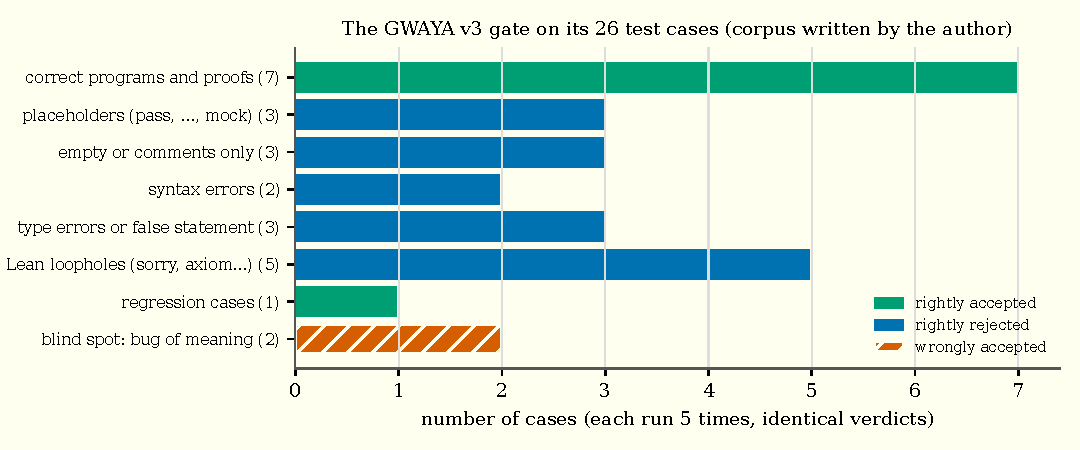
\includegraphics[width=\linewidth]{figures/c18_portail}
\caption{The 26 test cases of GWAYA~v3, counted from the published results file. Everything is right except the two
expected blind spots: code that does something other than intended, accepted because it is well formed.}
\label{fig:c18}
\end{figure}
